% verso e anverso:
% \documentclass[12pt,openright,twoside,a4paper,english]{abntex2}
% apenas verso:	
\documentclass[12pt,oneside,a4paper,english]{abntex2} 

\usepackage[alf]{abntex2cite}	% Citações padrão ABNT
\usepackage{listings}
\usepackage{float}
\usepackage{cmap}				% Mapear caracteres especiais no PDF
\usepackage{lmodern}			% Usa a fonte Latin Modern			
\usepackage[T1]{fontenc}		% Selecao de codigos de fonte.
\usepackage[utf8]{inputenc}		% Codificacao do documento (conversão automática dos acentos)
\usepackage{lastpage}			% Usado pela Ficha catalográfica
\usepackage{indentfirst}		% Indenta o primeiro parágrafo de cada seção.
\usepackage{color}				% Controle das cores
\usepackage{graphicx}			% Inclusão de gráficos
\usepackage{pdfpages}
\usepackage{tikz}
\usetikzlibrary{automata,positioning}
\usepackage{mathtools}

\definecolor{blue}{RGB}{41,5,195} % alterando o aspecto da cor azul

\makeatletter
\hypersetup{
    %pagebackref=true,
    pdftitle={\@title}, 
    pdfauthor={\@author},
    pdfsubject={\@title},
    pdfcreator={\imprimirpreambulo},
    pdfkeywords={Linguagens}{Compiladores}{Implementação do Reconhecedor Sintático}, 
    colorlinks=true,       		% false: boxed links; true: colored links
    linkcolor=blue,          	% color of internal links
    citecolor=blue,        		% color of links to bibliography
    filecolor=magenta,      		% color of file links
    urlcolor=blue,
    bookmarksdepth=4
}
\makeatother

\autor{Gustavo P. Gouveia (6482819), Victor Lassance (6431325)}
\title{Relatório de Compiladores\\Terceira Etapa\\Implementação do Reconhecedor Sintático\\Linguagem de programação \underline{CZAR}}
\orientador[Professor:]{Ricardo Luis de Azevedo da Rocha}
\preambulo{Texto apresentado à Escola Politécnica da Universidade de São Paulo como requisito para a aprovação na disciplina Linguagens e Compiladores no quinto módulo acadêmico do curso de graduação em Engenharia de Computação, junto ao Departamento de Engenharia de Computação e Sistemas Digitais (PCS).}
\instituicao{%
	Universidade de São Paulo
	\par
	Escola Politécnica
	\par
	Engenharia de Computação - Curso Cooperativo}
\local{São Paulo}
\data{2013}
\tipotrabalho{PCS2056 - Linguagens e Compiladores}

\setlength{\parindent}{1.3cm} % O tamanho do parágrafo
\setlength{\parskip}{0.2cm}  % Controle do espaçamento entre um parágrafo e outro

\makeindex

\begin{document}

\frenchspacing % Retira espaço extra obsoleto entre as frases.

\imprimirfolhaderosto

\clearpage
\begin{resumo}
	% !TEX encoding = UTF-8 Unicode
Este trabalho descreve a concepção e o desenvolvimento de um compilador utilizando a linguagem C. O escopo do compilador se limita a casos mais simples, porém simbólicos, e que servem ao aprendizado do processo de criação e teste de um compilador completo. A estrutura da linguagem escolhida para ser implementada se assemelha a própria estrutura do C, por facilidade de compreensão.

\vspace{\onelineskip}
    
\noindent
\textbf{Palavras-chaves}: Linguagens, Compiladores, Analisador Léxico.

\end{resumo}

\tableofcontents

\textual

\chapter{Introdução}
\label{chap:introducao}
	% !TEX encoding = UTF-8 Unicode

Este projeto tem como objetivo a construção de um compilador de um só passo, dirigido por sintaxe, com analisador e reconhecedor sintático baseado em autômato de pilha estruturado.

Em um primeiro momento, foi definida uma linguagem de programação e identificados os tipos de átomos. Para cada átomo foi escrito uma gramática linear representativa da sua lei de formação e um reconhecedor para o átomo. Desse modo, as gramáticas assim escritas foram unidas e convertidas em um autômato finito, o qual foi transformado em um transdutor e implementado como sub-rotina, dando origem ao analisador léxico propriamente dito. Também foi criada uma função principal para chamar o analisador léxico e possibilitar o seu teste.

Durante a segunda etapa, a sintaxe da linguagem, denonimada por nós de CZAR, foi definida formalmente a partir de uma definição informal e de exemplos de programas que criamos, misturando palavras-chave e conceitos de diferentes linguagens de programação. As três principais definições foram escritas na notação BNF\footnote{Ver http://en.wikipedia.org/wiki/Backus\_Naur\_Form}, Wirth\footnote{Ver http://en.wikipedia.org/wiki/Wirth\_syntax\_notation} e com diagramas de sintaxe.

Na terceira etapa, implementamos o módulo referente à parte sintática para a nossa linguagem. O analisador sintático construído obtém uma cadeia de \emph{tokens} proveniente do analisador léxico, e verifica se a mesma pode ser gerada pela gramática da linguagem e, com isso, constrói a árvore sintática \cite{alfred1986compilers}.

Para a quarta entrega, focamos no ambiente de execução. O compilador por nós criado tem como linguagem de saída um programa que é executado na máquina virtual conhecida como Máquina de von Neumann (MVN).

Já durante as duas últimas entregas, complementamos a especificação do código gerado pelo compilador e das rotinas do ambiente de execução da nossa linguagem de alto nível, a CZAR. Além disso, buscamos integrar as rotinas semânticas no reconhecedor sintático de forma a permitir a geração de código e finalizar o compilador.

Como material de consulta, além de sites sobre o assunto e das aulas ministradas, foi utilizado o livro indicado pelo professor no começo das aulas \cite{intro-compiladores}, para pesquisa de conceitos e possíveis implementações.

O documento apresenta a seguir o processo completo de desenvolvimento de um compilador, desde a definição formal da linguagem, passando pelo analisador léxico, reconhecedor sintático, pela definição do ambiente de execução e das rotinas semânticas, terminando com um exemplo de programa traduzido.


\chapter{Descrição Atualizada da Linguagem em Wirth}
\label{chap:wirth}
	% !TEX encoding = UTF-8 Unicode

\lstinputlisting[frame=single,numbers=left,breaklines=true,basicstyle=\ttfamily\scriptsize]{files/WIRTH.txt}


\chapter{Lista de Submáquinas do APE}
\label{chap:lista-submaquinas}
	% !TEX encoding = UTF-8 Unicode

\section{Lista de Transições}
\label{chap:lista-transicoes}
	% !TEX encoding = UTF-8 Unicode

\textbf{Autômato Finito Determinístico Mínimo da submáquina ATOMO-COND:}
\lstinputlisting[frame=single,numbers=left,breaklines=true,basicstyle=\ttfamily\scriptsize]{files/submaquinas/ATOMO-COND.mdfa}

\textbf{Autômato Finito Determinístico Mínimo da submáquina \emph{ATOMO}:}
\lstinputlisting[frame=single,numbers=left,breaklines=true,basicstyle=\ttfamily\scriptsize]{files/submaquinas/ATOMO.mdfa}

\textbf{Autômato Finito Determinístico Mínimo da submáquina \emph{BOTH}:}
\lstinputlisting[frame=single,numbers=left,breaklines=true,basicstyle=\ttfamily\scriptsize]{files/submaquinas/BOTH.mdfa}

\textbf{Autômato Finito Determinístico Mínimo da submáquina \emph{COND-TERM}:}
\lstinputlisting[frame=single,numbers=left,breaklines=true,basicstyle=\ttfamily\scriptsize]{files/submaquinas/COND-TERM.mdfa}

\textbf{Autômato Finito Determinístico Mínimo da submáquina \emph{COND}:}
\lstinputlisting[frame=single,numbers=left,breaklines=true,basicstyle=\ttfamily\scriptsize]{files/submaquinas/COND.mdfa}

\textbf{Autômato Finito Determinístico Mínimo da submáquina \emph{DECLS-GLOBAIS}:}
\lstinputlisting[frame=single,numbers=left,breaklines=true,basicstyle=\ttfamily\scriptsize]{files/submaquinas/DECLS-GLOBAIS.mdfa}

\textbf{Autômato Finito Determinístico Mínimo da submáquina \emph{DEF-MAIN}:}
\lstinputlisting[frame=single,numbers=left,breaklines=true,basicstyle=\ttfamily\scriptsize]{files/submaquinas/DEF-MAIN.mdfa}

\textbf{Autômato Finito Determinístico Mínimo da submáquina \emph{DEF-PROCS-FUNCS}:}
\lstinputlisting[frame=single,numbers=left,breaklines=true,basicstyle=\ttfamily\scriptsize]{files/submaquinas/DEF-PROCS-FUNCS.mdfa}

\textbf{Autômato Finito Determinístico Mínimo da submáquina \emph{EXPR}:}
\lstinputlisting[frame=single,numbers=left,breaklines=true,basicstyle=\ttfamily\scriptsize]{files/submaquinas/EXPR.mdfa}

\textbf{Autômato Finito Determinístico Mínimo da submáquina \emph{FUNCTION-CALL}:}
\lstinputlisting[frame=single,numbers=left,breaklines=true,basicstyle=\ttfamily\scriptsize]{files/submaquinas/FUNCTION-CALL.mdfa}

\textbf{Autômato Finito Determinístico Mínimo da submáquina \emph{IMPORTS}:}
\lstinputlisting[frame=single,numbers=left,breaklines=true,basicstyle=\ttfamily\scriptsize]{files/submaquinas/IMPORTS.mdfa}

\textbf{Autômato Finito Determinístico Mínimo da submáquina \emph{INSTR-SEM-RET}:}
\lstinputlisting[frame=single,numbers=left,breaklines=true,basicstyle=\ttfamily\scriptsize]{files/submaquinas/INSTR-SEM-RET.mdfa}

\textbf{Autômato Finito Determinístico Mínimo da submáquina \emph{LIST-PARAMS}:}
\lstinputlisting[frame=single,numbers=left,breaklines=true,basicstyle=\ttfamily\scriptsize]{files/submaquinas/LIST-PARAMS.mdfa}

\textbf{Autômato Finito Determinístico Mínimo da submáquina \emph{OPER-ATRIB}:}
\lstinputlisting[frame=single,numbers=left,breaklines=true,basicstyle=\ttfamily\scriptsize]{files/submaquinas/OPER-ATRIB.mdfa}

\textbf{Autômato Finito Determinístico Mínimo da submáquina \emph{PROGRAM}:}
\lstinputlisting[frame=single,numbers=left,breaklines=true,basicstyle=\ttfamily\scriptsize]{files/submaquinas/PROGRAM.mdfa}

\textbf{Autômato Finito Determinístico Mínimo da submáquina \emph{TERM}:}
\lstinputlisting[frame=single,numbers=left,breaklines=true,basicstyle=\ttfamily\scriptsize]{files/submaquinas/TERM.mdfa}

\textbf{Autômato Finito Determinístico Mínimo da submáquina \emph{VARIDENT}:}
\lstinputlisting[frame=single,numbers=left,breaklines=true,basicstyle=\ttfamily\scriptsize]{files/submaquinas/VARIDENT.mdfa}


\section{Lista de Autômatos}
\label{chap:lista-automatos}
	% !TEX encoding = UTF-8 Unicode

\begin{itemize}

	\item ATOMO-COND:
	\begin{figure}[H]
		\centering 
		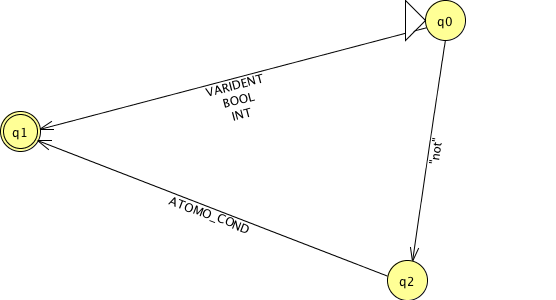
\includegraphics[width=0.8\textwidth]{images/submaquinas/ATOMO-COND.png}  
		\caption{Autômato ATOMO-COND}
	\end{figure}
	
	\item ATOMO:
	\begin{figure}[H]
		\centering 
		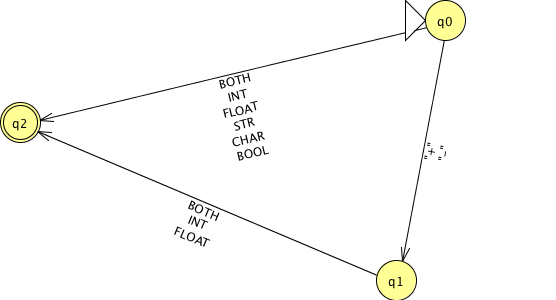
\includegraphics[width=0.8\textwidth]{images/submaquinas/ATOMO.png}  
		\caption{Autômato ATOMO}
	\end{figure}
	
	\item BOTH:
	\begin{figure}[H]
		\centering 
		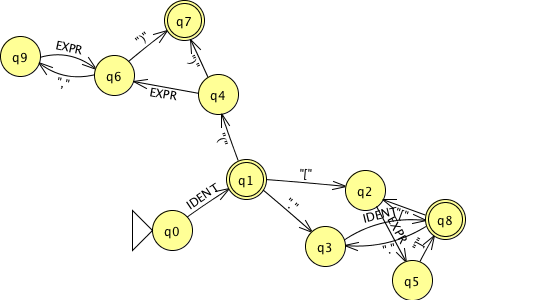
\includegraphics[width=0.8\textwidth]{images/submaquinas/BOTH.png}  
		\caption{Autômato BOTH}
	\end{figure}
	
	\item COND-TERM:
	\begin{figure}[H]
		\centering 
		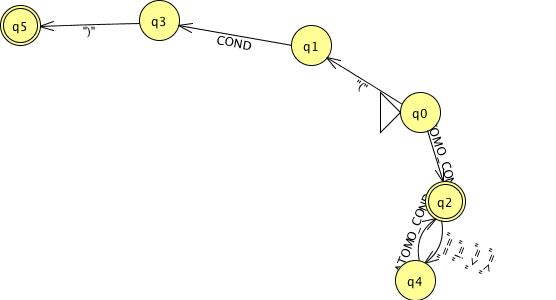
\includegraphics[width=0.8\textwidth]{images/submaquinas/COND-TERM.png}  
		\caption{Autômato COND-TERM}
	\end{figure}
	
	\item COND:
	\begin{figure}[H]
		\centering 
		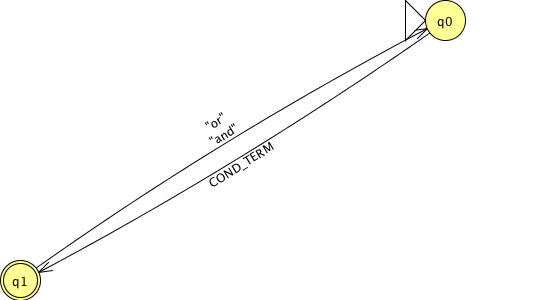
\includegraphics[width=0.8\textwidth]{images/submaquinas/COND.png}  
		\caption{Autômato COND}
	\end{figure}
	
	\item DECLS-GLOBAIS:
	\begin{figure}[H]
		\centering 
		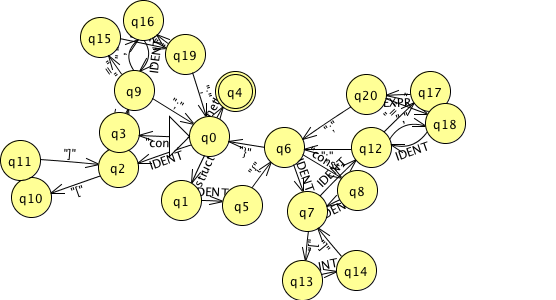
\includegraphics[width=0.8\textwidth]{images/submaquinas/DECLS-GLOBAIS.png}  
		\caption{Autômato DECLS-GLOBAIS}
	\end{figure}
	
	\item DEF-MAIN:
	\begin{figure}[H]
		\centering 
		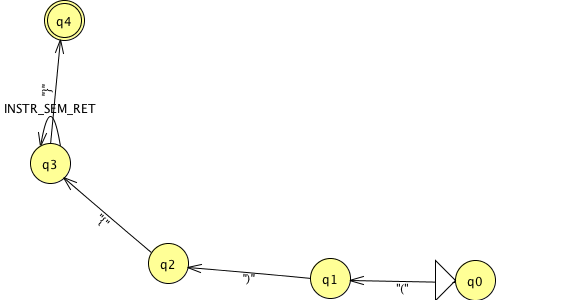
\includegraphics[width=0.8\textwidth]{images/submaquinas/DEF-MAIN.png}  
		\caption{Autômato DEF-MAIN}
	\end{figure}
	
	\item DEF-PROCS-FUNCS:
	\begin{figure}[H]
		\centering 
		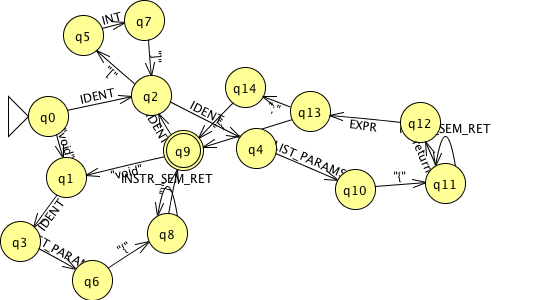
\includegraphics[width=0.8\textwidth]{images/submaquinas/DEF-PROCS-FUNCS.png}  
		\caption{Autômato DEF-PROCS-FUNCS}
	\end{figure}
	
	\item EXPR:
	\begin{figure}[H]
		\centering 
		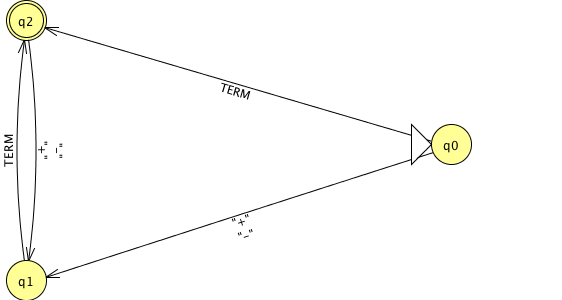
\includegraphics[width=0.8\textwidth]{images/submaquinas/EXPR.png}  
		\caption{Autômato EXPR}
	\end{figure}
	
	\item FUNCTION-CALL:
	\begin{figure}[H]
		\centering 
		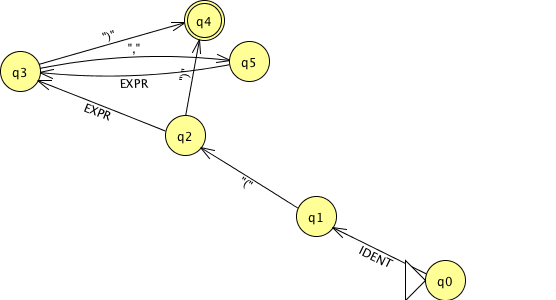
\includegraphics[width=0.8\textwidth]{images/submaquinas/FUNCTION-CALL.png}  
		\caption{Autômato FUNCTION-CALL}
	\end{figure}
	
	\item IMPORTS:
	\begin{figure}[H]
		\centering 
		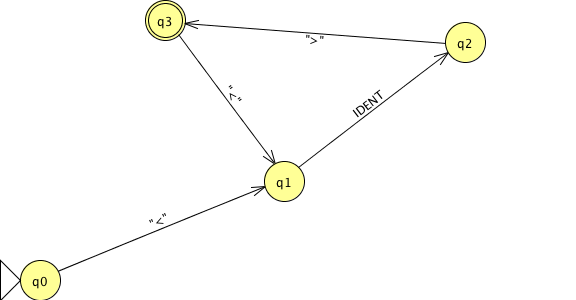
\includegraphics[width=0.8\textwidth]{images/submaquinas/IMPORTS.png}  
		\caption{Autômato IMPORTS}
	\end{figure}
	
	\item INSTR-SEM-RET:
	\begin{figure}[H]
		\centering 
		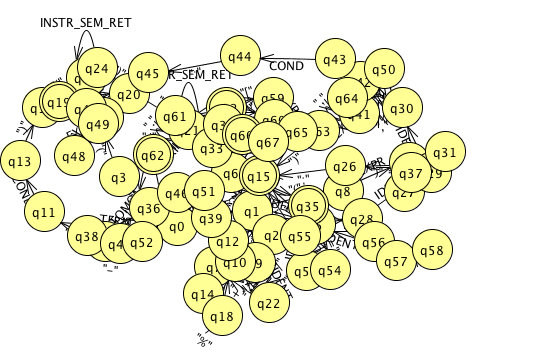
\includegraphics[width=1.0\textwidth]{images/submaquinas/INSTR-SEM-RET.png}  
		\caption{Autômato INSTR-SEM-RET}
	\end{figure}
	
	\item LIST-PARAMS:
	\begin{figure}[H]
		\centering 
		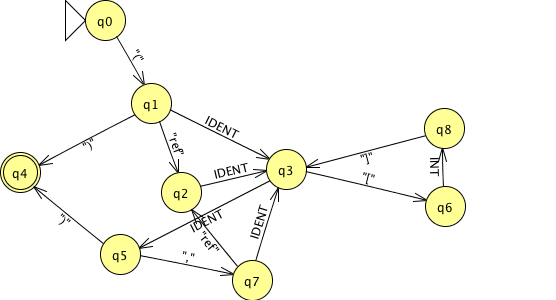
\includegraphics[width=0.8\textwidth]{images/submaquinas/LIST-PARAMS.png}  
		\caption{Autômato LIST-PARAMS}
	\end{figure}
	
	\item OPER-ATRIB:
	\begin{figure}[H]
		\centering 
		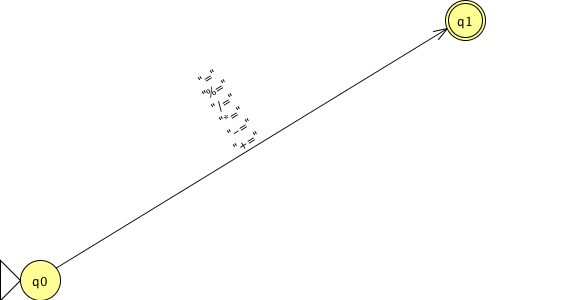
\includegraphics[width=0.8\textwidth]{images/submaquinas/OPER-ATRIB.png}  
		\caption{Autômato OPER-ATRIB}
	\end{figure}
	
	\item PROGRAM:
	\begin{figure}[H]
		\centering 
		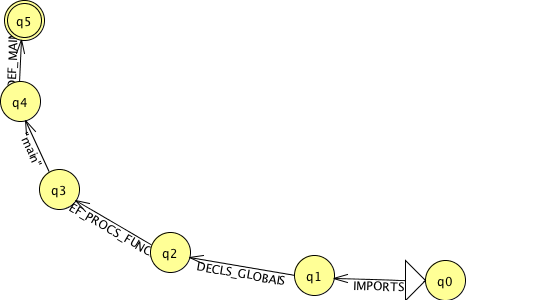
\includegraphics[width=0.8\textwidth]{images/submaquinas/PROGRAM.png}  
		\caption{Autômato PROGRAM}
	\end{figure}
	
	\item TERM:
	\begin{figure}[H]
		\centering 
		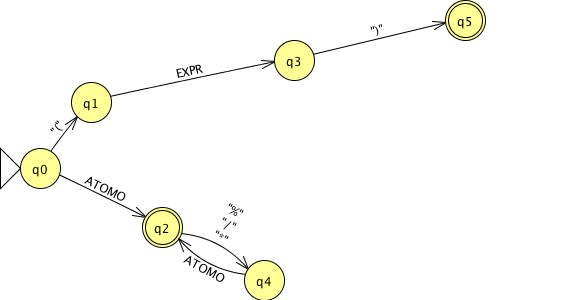
\includegraphics[width=0.8\textwidth]{images/submaquinas/TERM.png}  
		\caption{Autômato TERM}
	\end{figure}
	
	\item VARIDENT:
	\begin{figure}[H]
		\centering 
		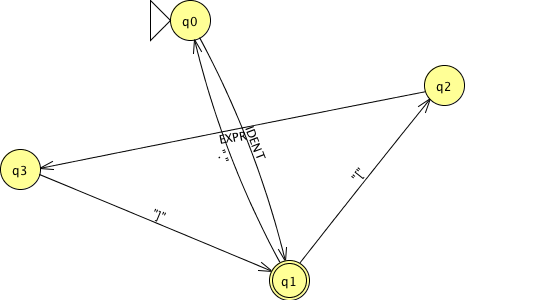
\includegraphics[width=0.8\textwidth]{images/submaquinas/VARIDENT.png}  
		\caption{Autômato VARIDENT}
	\end{figure}

\end{itemize}



\chapter{Exemplos Atualizados de Programas na Linguagem \emph{CZAR}}
\label{chap:exemplo-programa}
	% !TEX encoding = UTF-8 Unicode

\section{Exemplo Geral}
\label{chap:exemplo-geral}
	% !TEX encoding = UTF-8 Unicode

\lstinputlisting[frame=single,numbers=left,breaklines=true,morekeywords={main,const,int,char,string,void,return,for,struct,if,ref,float,else,and,or,not,true,false},basicstyle=\ttfamily\scriptsize]{files/exemplo-programa-geral.czar}


\section{Exemplo Fatorial}
\label{chap:exemplo-fatorial}
	% !TEX encoding = UTF-8 Unicode

\lstinputlisting[frame=single,numbers=left,breaklines=true,morekeywords={main,const,int,char,string,void,return,for,struct,if,ref,float,else,and,or,not,true,false}]{files/exemplo-programa-fatorial.czar}



\chapter{Comentários sobre a Implementação do Reconhecedor Sintático}
\label{chap:comentarios-implementacao}
	% !TEX encoding = UTF-8 Unicode

TODO:Gustavo explicar como o analisador sintático foi implementado e integrado ao compilador


\bibliography{bibliografia}

\end{document}
